
\begin{frame}[c]
  \frametitle{Case III : Solubility Coefficient}
The reference solubilities for each element were multiplied by the multiplier 
for each simulation group. This technique preserved relative solubility among 
  elements. 

\begin{table}[ht!]
\centering
\footnotesize{
\begin{tabular}{|l|l|l|r|r|}
\multicolumn{5}{c}{\textbf{Simulation Cases}}\\
\hline
\textbf{Case} & \textbf{Parameter} & \textbf{Units} & \textbf{Min. Value} & \textbf{Max. Value}\\
\hline
III   & $S_i$        & $[mol\cdot m^{-3}]$       & $(1\times10^{-9})\langle S_i\rangle $    &  $(5\times10^{10})\langle S_i\rangle $ \\
\hline
\end{tabular}
\caption{Case III varied a solubility factor across many magnitudes. This single parameter simulation case had 40 simulation 
groups of 100 realizations each.}
\label{tab:Cases}
}
\end{table}


\end{frame}

\begin{frame}[c]
  \frametitle{Case III : Solubility Coefficient}


\begin{figure}[ht]
\centering
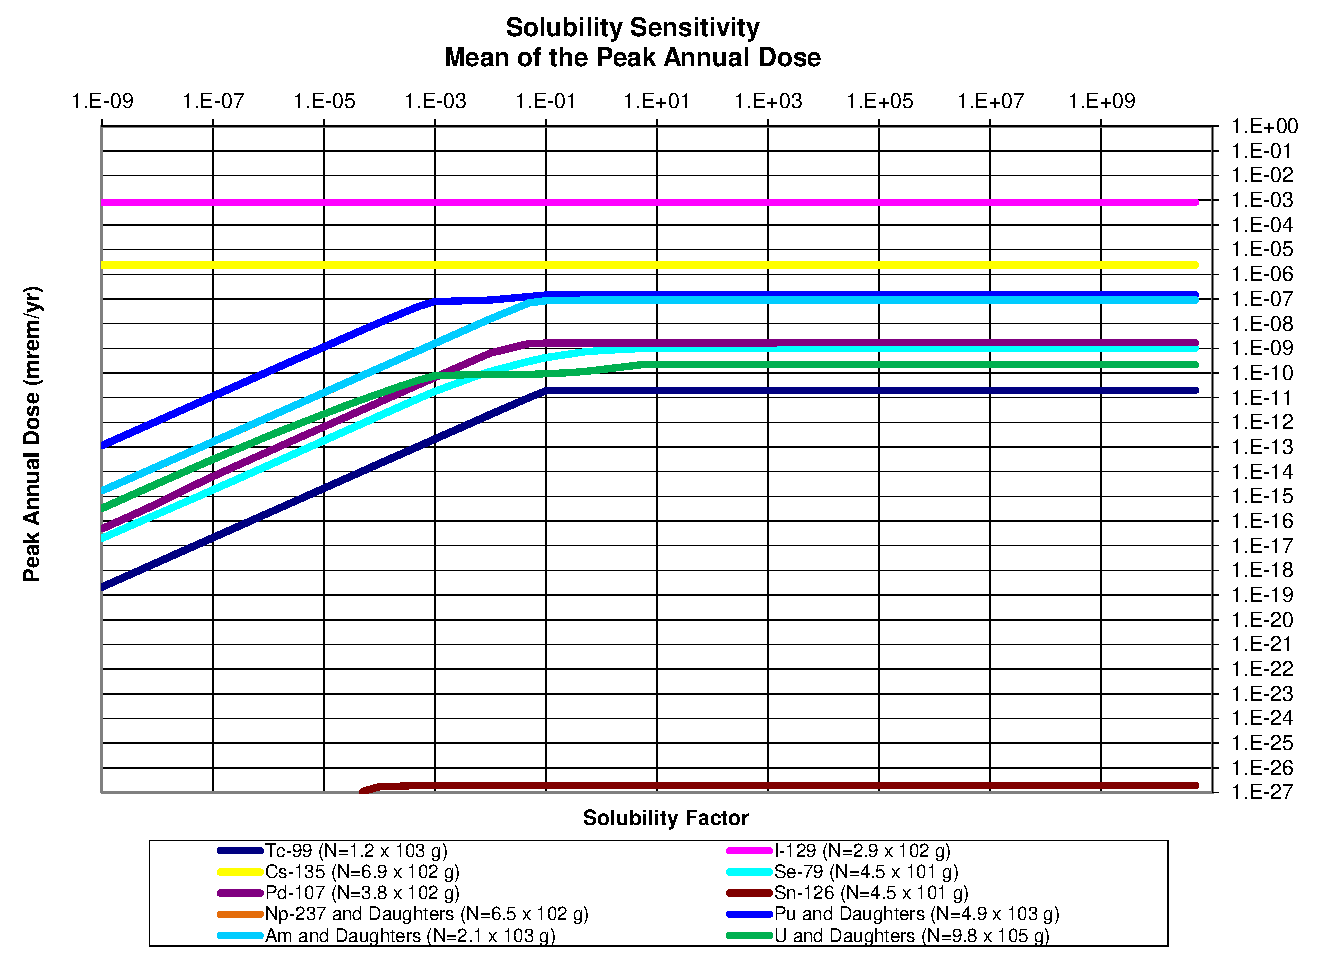
\includegraphics[width=0.8\textwidth]{Solubility/Solubility_Summary_SolFactor.eps}
\caption{
The peak annual dose due to an inventory, $N$, of each isotope.
For solubility constants lower than the inventory threshold, the relationship between peak 
annual dose and solubility limit is strong.}
\label{fig:SolSumFactor}
\end{figure}
\end{frame}

